\documentclass[10pt]{article}

\usepackage[a4paper, margin=2.6cm]{geometry}
\usepackage{amsmath}
\usepackage{booktabs}
\usepackage{graphicx}
\usepackage{caption}
\usepackage{float}
\usepackage{microtype}
\usepackage{algorithm}
\usepackage[noend]{algpseudocode}
\usepackage{xcolor}
\usepackage[hidelinks]{hyperref}

\graphicspath{{../../plots/}}
\captionsetup{font=small, labelfont=bf}

% let floats fill the top of a page and leave the rest for text
\renewcommand{\topfraction}{0.95}
\renewcommand{\bottomfraction}{0.0}
\renewcommand{\textfraction}{0.08}
\renewcommand{\floatpagefraction}{0.85}
\setcounter{topnumber}{3}
\setlength{\textfloatsep}{18pt plus 4pt minus 4pt}

\algrenewcommand\algorithmicindent{1.1em}
\makeatletter
\renewcommand{\ALG@name}{Kernel}
\makeatother

\newcommand{\e}[1]{\times 10^{#1}}
\newcommand{\rd}{\texttt{ragged\_dot}}

\title{A Fused Pallas Kernel for the Mixture-of-Experts MLP}
\author{Hyeonseok Jung}
\date{}

\begin{document}
\maketitle

\section{Problem statement}

The expert MLP of a mixture-of-experts layer computes
\begin{equation}
  y[i] = \mathrm{down}[g(i)]^{\top}
         \bigl(\, \mathrm{swish}(x[i]\,\mathrm{gate}[g(i)]) \odot
         (x[i]\,\mathrm{up}[g(i)]) \,\bigr),
  \label{eq:op}
\end{equation}
where $x$ is $(m, d)$, $\mathrm{up}$ and $\mathrm{gate}$ are $(e, d, f)$,
$\mathrm{down}$ is $(e, f, d)$, and $g(i)$ is the expert assigned to token
$i$. Rows arrive sorted by expert, so the assignment is given by a vector of
$e$ group sizes summing to $m$. The router, the sort, the scatter back to
token order, and biases are outside the scope of this report. Written as
three \texttt{jax.lax.ragged\_dot} calls, this lands two $(m, f)$
intermediates in HBM and reads them back, so $6mf$ elements of intermediate
activations are communicated through memory between the three matmuls. I
fuse the up, gate, and down projections into a single Pallas kernel that
keeps those intermediates in VMEM. Every measurement below compares that
kernel against the reference on one TPU v5e core under JAX 0.6.2, in
bfloat16.

\section{The fused kernel}

The kernel evaluates
\begin{equation}
  y[m, j] = \sum_i
    \Bigl( \bigl(\textstyle\sum_k x[m,k]\,\mathrm{up}_e[k,i]\bigr)
    \odot \mathrm{swish}\bigl(\textstyle\sum_k x[m,k]\,\mathrm{gate}_e[k,i]\bigr) \Bigr)
    \mathrm{down}_e[i,j]
\end{equation}
over a four-dimensional \texttt{pltpu.emit\_pipeline} grid $(m, i, j, k)$,
where $m$ indexes tiles of rows, $i$ the hidden dimension $f$, $j$ the
output dimension $d$, and $k$ the contracted input dimension $d$, with block
sizes $(b_m, b_i, b_j, b_k)$. Write $I = f/b_i$, $J = d/b_j$, and
$K = d/b_k$ for the number of steps along each axis, and $e$ for the expert
owning row tile $m$.

\begin{algorithm}[H]
\caption{Fused expert MLP, one grid step per innermost iteration.}
\begin{algorithmic}[1]
\For{$m \gets 0$ \textbf{to} row tiles $-\,1$}
  \For{$i \gets 0$ \textbf{to} $I - 1$}
    \For{$j \gets 0$ \textbf{to} $J - 1$}
      \For{$k \gets 0$ \textbf{to} $K - 1$}
        \If{$i = 0$ \textbf{and} $j = 0$ \textbf{and} $k = 0$}
          \State $\mathrm{acc} \gets 0$
          \Comment{$(b_m, d)$ output accumulator}
        \EndIf
        \If{$j = 0$ \textbf{and} $k = 0$}
          \State $a \gets 0$, \; $g \gets 0$
          \Comment{$(b_m, b_i)$ hidden accumulators}
        \EndIf
        \If{$j = 0$}
          \State $a \gets a + x[m, k] \cdot \mathrm{up}_e[k, i]$
          \State $g \gets g + x[m, k] \cdot \mathrm{gate}_e[k, i]$
        \EndIf
        \If{$k = K - 1$}
          \State $\mathrm{acc}[:, j] \gets \mathrm{acc}[:, j]
                 + \bigl(a \odot \mathrm{swish}(g)\bigr) \cdot \mathrm{down}_e[i, j]$
        \EndIf
        \If{$i = I - 1$ \textbf{and} $k = K - 1$}
          \State $\mathrm{out}[m, j] \gets \mathrm{acc}[:, j]$
        \EndIf
      \EndFor
    \EndFor
  \EndFor
\EndFor
\end{algorithmic}
\end{algorithm}

Two float32 accumulators of shape $(b_m, b_i)$ hold the up and gate partial
sums for the current $(m, i)$ pair, and one of shape $(b_m, d)$ holds the
output partial sums for the row tile. The combination
$a \odot \mathrm{swish}(g)$ is formed on the accumulator tile and fed
straight into the down matmul, so neither it nor either factor ever reaches
HBM. The kernel accumulates in float32 throughout, where the reference
rounds each ragged dot's output to bfloat16.

The ragged structure enters through the block index maps, which return the
expert of the current row tile from a small SMEM array. For one expert to
own each tile, group boundaries must fall on multiples of $b_m$, so I pad
$x$ with zero rows before the call and gather the rows back afterwards; the
row-tile count $\sum_j \lceil s_j / b_m \rceil$ is data-dependent and is
passed in as an operand. Both the padding and the gather back are timed as
part of the kernel in every measurement below.

\section{Results}

Every measurement uses the same block-size rule, derived from the shape and
never tuned per point: $b_m = \min(256,\, m/2e)$, $b_i = \min(1024,\, f/4)$,
$b_j = \min(1024,\, d)$, and $b_k = \min(512,\, d/2)$. Reported rates are $6mdf$ divided by the measured time, and the kernel's
output matches the reference to a relative and absolute tolerance of
$2\e{-2}$ at every point below. At the reference shape
$(m, d, f, e) = (16384, 1024, 4096, 8)$ the fused kernel is $1.59\times$
faster, 3.09\,ms against 4.90\,ms. The removed traffic accounts for all of
that. The reference's elementwise stage does no matmul work and streams
$3mf$ elements in 946\,\textmu s, so the $6mf$ elements the fusion
eliminates are worth 1.89\,ms at the same rate, against a measured saving of
1.82\,ms.

\subsection{Shape sweeps}

\begin{figure}[t]
\centering
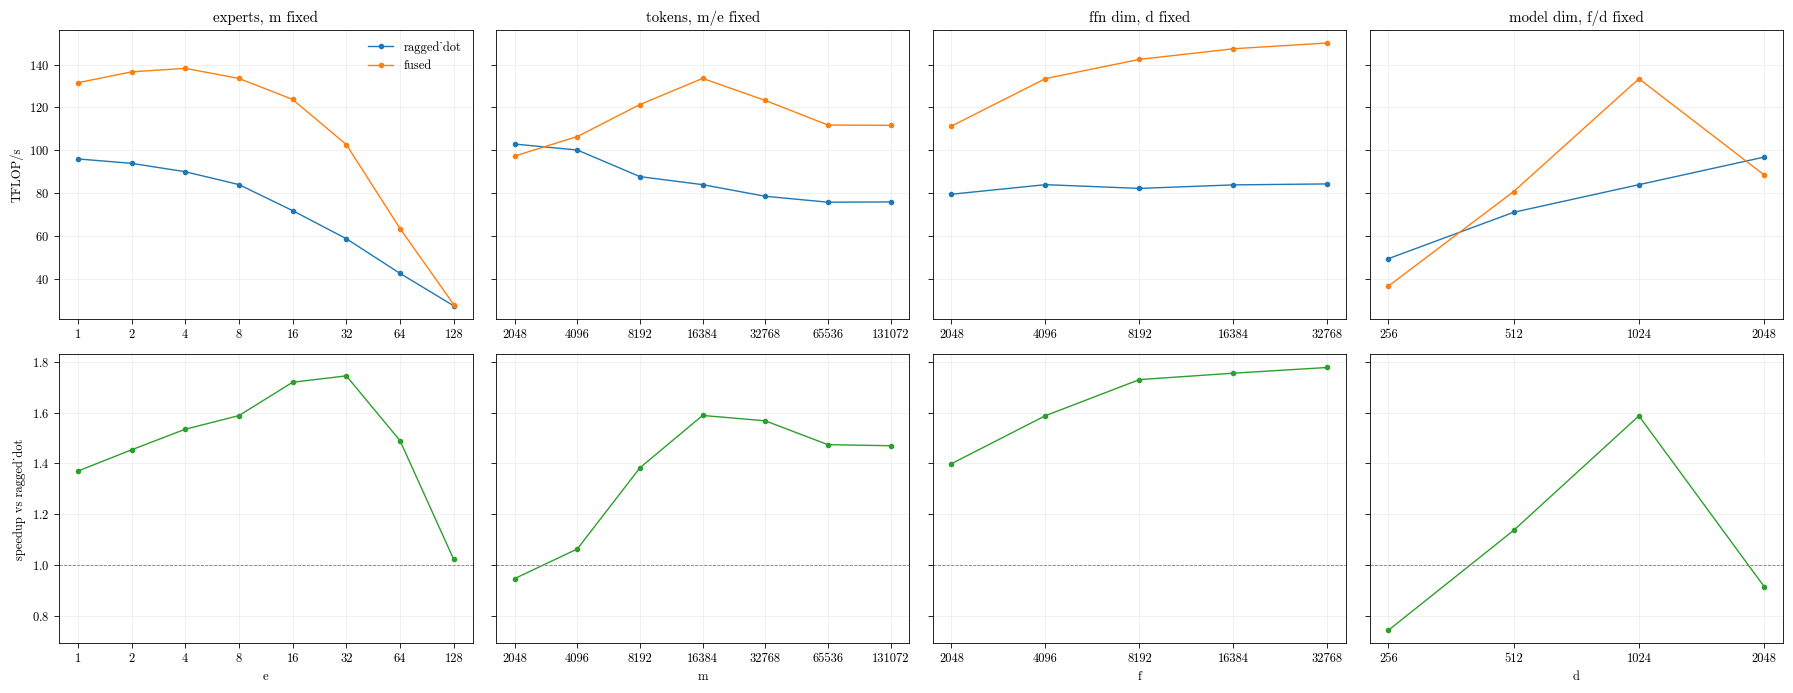
\includegraphics[width=\textwidth]{moe_optimization/hyperparam_sweep.png}
\caption{Shape sweeps: (a) expert count, (b) token count, (c) hidden
dimension, (d) model dimension. Top row, achieved rate; bottom row, their
ratio. One parameter doubles per point, the rest held at the reference shape
$(m, d, f, e) = (16384, 1024, 4096, 8)$. In (b) each expert keeps 2048 rows;
in (d) $f/d$ stays at 4.}
\label{fig:sweeps}
\end{figure}

The expert count sweep (Figure~\ref{fig:sweeps}a) rises to a peak and then
falls. The speedup improves from 1.37 at one expert to 1.75 at 32 experts,
then drops to 1.03 at 128. The token count is fixed, so the mean
group size is $m/e$ and it shrinks as experts are added. Each expert's three
weight slabs are read to serve only the rows of its own group, which makes
the arithmetic intensity with respect to weight traffic equal to the group
size in FLOPs per byte. Once that number is small, the reference and the
fused kernel both spend their time streaming those weights, and their rates
converge. The fusion
removes communication between operations. It cannot remove traffic that the
operation itself requires.

The token count sweep (Figure~\ref{fig:sweeps}b) holds the group size at
2048 rows and grows the expert count with the token count. The speedup rises
from 0.95 at $m = 2048$ to 1.59 at $m = 16384$, then settles near 1.47. The
kernel is slower only at the smallest point, where one expert and 2048 rows
give 8 row tiles. I did not profile that shape, so I cannot divide the loss
between the pipeline's fill and drain, the padding gathers, and fixed launch
cost.

The hidden dimension sweep (Figure~\ref{fig:sweeps}c) is the regime the
fusion targets. With $d$ fixed at 1024, the speedup rises monotonically from
1.40 at $f = 2048$ to 1.78 at $f = 32768$. The reference holds a flat rate
across the whole range, because its intermediate traffic and its FLOPs both
grow in proportion to $f$ and the ratio between them does not change. The
fused kernel does not pay that traffic, so its rate climbs instead.

The model dimension sweep (Figure~\ref{fig:sweeps}d) peaks in the middle of
its range. The speedup is 1.59 at $d = 1024$, 0.75 at $d = 256$, and 0.91 at
$d = 2048$. Both ends are failures of the block-size rule rather than of the
fusion. At $d = 256$ the rule yields
tiles that are too small for the MXU. At $d = 2048$ it gives the first shape
in any sweep with $b_j < d$, which makes the kernel run the full $k$ loop
once per $j$ block while only the last step does work.

\subsection{Aspect ratio at equal FLOPs}

The $f$ sweep raises $f/d$ and the total work together, so it cannot
separate the two. Holding $df$ fixed separates them. The three points in
Figure~\ref{fig:ratio} share $m$, $e$, and FLOP count, and differ only in
the shape of the MLP. Only three such points satisfy $f > d$ with $b_k$ a
multiple of 128.

\begin{figure}[t]
\centering
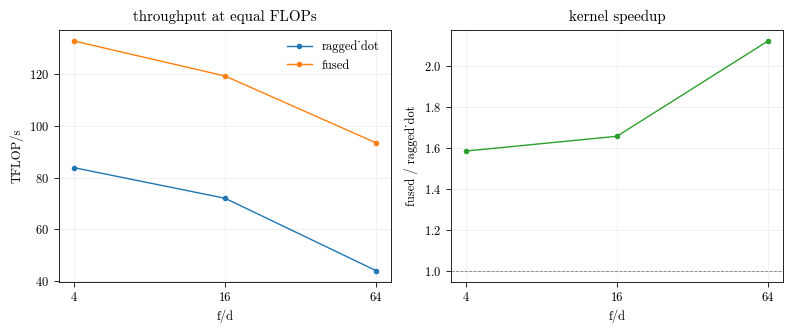
\includegraphics[width=0.62\textwidth]{moe_optimization/fixed_flops.png}
\caption{Constant FLOP count: (a) achieved throughput, (b) speedup. All
three points are $m = 16384$, $e = 8$, $df = 2^{22}$.}
\label{fig:ratio}
\end{figure}

\begin{table}[H]
\centering
\small
\begin{tabular}{ccrrrr}
\toprule
$f/d$ & $(d, f)$ & \rd{} & fused & speedup & intermediates \\
\midrule
4  & (1024, 4096)  & 83.7 & 132.8 & 1.59 & 805\,MB \\
16 & (512, 8192)   & 72.1 & 119.2 & 1.66 & 1.61\,GB \\
64 & (256, 16384)  & 43.9 & \phantom{0}93.3 & 2.12 & 3.22\,GB \\
\bottomrule
\end{tabular}
\caption{The equal-FLOPs comparison. Rates are TFLOP/s; the last column is
the intermediate traffic the reference moves and the fused kernel does
not.}
\label{tab:ratio}
\end{table}

The speedup rises from 1.59 to 2.12, and the mechanism is the last column of
Table~\ref{tab:ratio}. At a fixed $df$ product the intermediate volume $mf$
grows as the square root of the aspect ratio, so each factor of four in
$f/d$ doubles the traffic the reference must move while its FLOPs and weight
traffic stay constant. The fused kernel also slows over the same range, because at
$d = 256$ its matmuls are much narrower in the contracted dimension. Its
rate falls by less than half as much as the reference's.

\subsection{Routing skew}

All measurements so far use balanced experts. Real routing does not produce
them, so I repeated the comparison with skewed assignments.
Figure~\ref{fig:skew} scales the router logits by a skew parameter, and
larger values concentrate tokens on fewer experts.

\begin{figure}[H]
\centering
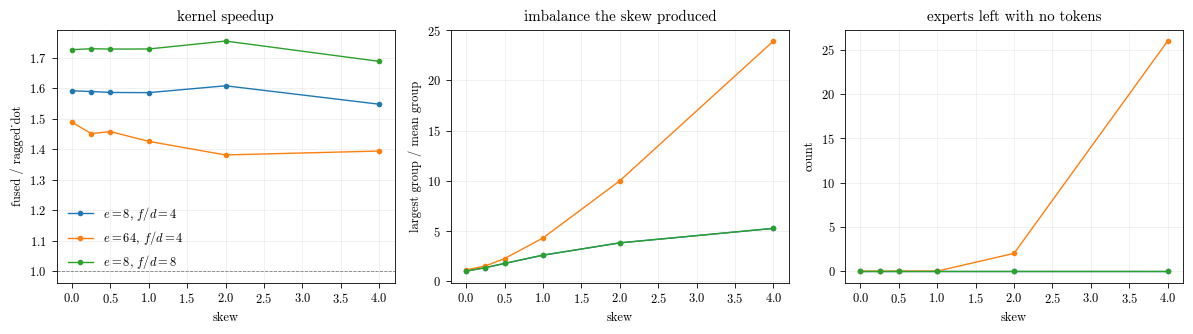
\includegraphics[width=\textwidth]{moe_optimization/skew.png}
\caption{Effect of routing skew: (a) speedup, (b) the imbalance the skew
produced, (c) experts left with no tokens. All three are $m = 16384$,
$d = 1024$. The two $e = 8$ configurations share a group-size distribution,
so their lines coincide in (b) and (c).}
\label{fig:skew}
\end{figure}

At eight experts the speedup barely moves, from 1.59 to 1.55 at $f/d = 4$,
while the largest group grows to 5.3 times the mean. At 64 experts it
degrades from 1.49 to 1.39 over a range where the largest group reaches 24
times the mean and 26 experts end up empty.

The difference is the padding tax. A group of $s$ rows costs
$\lceil s / b_m \rceil$ tiles, so the waste is at most $b_m - 1$ rows per
non-empty group and empty groups cost nothing. At eight experts the mean
group is 2048 rows against $b_m = 256$, so the waste is negligible. At 64
experts it is 256 rows against $b_m = 128$, and skew drives many groups
below a full tile. The degradation therefore follows the ratio of group size
to tile height.

\section{Conclusion}

The fusion removes the intermediate traffic and changes nothing else. A
speedup appears when that traffic was a large share of the reference's
runtime. It disappears when some other cost becomes the bottleneck. Four
conditions follow from the measurements.

\begin{itemize}
\itemsep2pt
  \item \textbf{$f$ larger than $d$.} The removed traffic scales with $mf$,
    while the input, the output, and the expert weights move either way. At
    equal FLOPs the speedup goes from 1.59 at $f/d = 4$ to 2.12 at
    $f/d = 64$.
  \item \textbf{Enough tokens per expert.} An expert's three weight slabs
    are $3df$ elements and they are read to serve only the rows routed to
    that expert, so the arithmetic done per weight byte read is exactly the
    group size. A small group means streaming a large weight matrix to do
    very little arithmetic with it. The reference and the fused kernel read
    the same weights, so both are then limited by that stream rather than by
    anything the fusion changes. At $e = 128$ the mean group is 128 rows,
    the two run at 28 TFLOP/s each, and the speedup falls to 1.03.
  \item \textbf{Groups no smaller than the tile height $b_m$.} A group of
    $s$ rows occupies $\lceil s / b_m \rceil$ whole tiles, so a group
    shorter than a tile pays for rows it does not have. Routing skew acts
    through this channel. It costs nothing at 8 experts, where groups are
    2048 rows against $b_m = 256$, and takes the speedup from 1.49 to 1.39
    at 64 experts.
  \item \textbf{Block sizes matched to the shape.} At $d = 256$ the rule
    gives tiles too small for the MXU and at $d = 2048$ it gives $b_j < d$,
    costing 0.75 and 0.91. These are failures of the rule, not of the
    fusion.
\end{itemize}

\end{document}
